$subject$=Физические основы компьютерных \\ и сетевых технологий
$teacher$=Лекции Герта А. В.
$date$=17.03.2025

\section{Лекция 6. Колебания}

$T = 2\pi \sqrt{LC}$ - формула Томпсона

Напряжение на конденсаторе меняется в такт с зарядом

$U_C(t) = \frac{q}{C} = \frac{q_{\max}}{C} \cos (\omega_0 t + \alpha) = U_{\max} \cos (\omega_0 t + \alpha)$

А сила тока опережает по фазе напряжение на конденсаторе на $\frac{\pi}{2}$

$I(t) = \frac{dq}{dt} = -\omega_0 q_{\max} \sin(\omega_0 t + \alpha) = I_{\max} \cos(\omega_0 t + \alpha + \frac{\pi}{2})$


$U_{\max} = \frac{1}{\omega_0 C} I_{\max} = \sqrt{\frac{L}{C}} I_{\max}$

$W_E = \frac{C U^2_C (t)}{2}$

$W_B = \frac{L I^2(t)}{2}$

\subsection{Вектор колебаний}

Сложение нескольких гармонических колебаний одного направления и одинаковой частоты облегчается, 
если изображать колебания графически в виде векторов на плоскости. Полученная таким способом схема называется 
векторной диаграммой.

% https://www.geogebra.org/calculator/jhshxnfd

\begin{wrapfigure}{R}{0pt}
    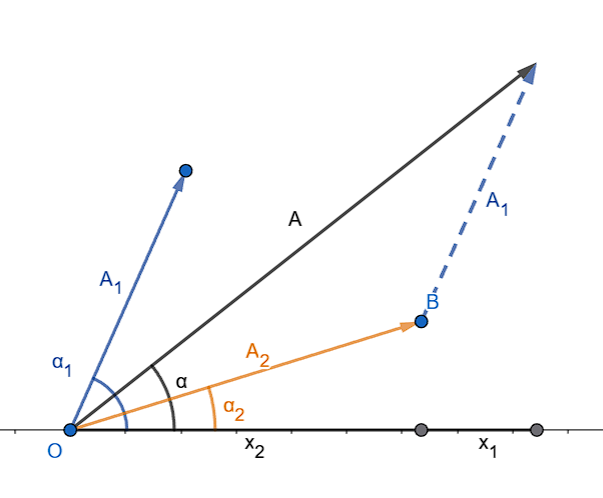
\includegraphics[width=6cm]{physics2/images/physics2_2025_03_17_1}
\end{wrapfigure}

Возьмем ось $Ox$, точку $O$, от оси с углом $\alpha$ отложим вектор длиной $A$. Если привести вектор
во вращение с угловой скоростью $\omega_0$, то проекция вектора будет перемещаться в по оси $Ox$ 
в пределах от $-A$ до $A$. Причем координата проекции будет изменяться по закону: $x(t) = A\cos (\omega_0 t + \alpha)$

Если два колебания представить с помощью векторов $A_1$ и $A_2$, то проекция суммы векторов $A$ на ось будет 
представлять сумму проекций. $A$ будет вращаться с той же частотой, что и $A_1$ и $A_2$

По геометрическим соображениям тангенс угла вектора $A$ $\alpha$ (также начальная фаза колебаний) равен 
$\tg \alpha = \frac{A_1 \sin \alpha_1 + A_2 \sin \alpha_2}{A_1 \cos \alpha_1 + A_2 \cos \alpha_2}$

Если частоты двух гармонических колебаний различны, то их сумма не будет являться гармоническим колебанием.
Но если колебания одного направления мало отличаются по частоте, то сумму колебаний можно рассматривать
как гармоническое колебание с пульсирующей амплитудой. Такое колебание называется биениями.

Рассмотрим одно колебание с частотой $\omega$, другое колебание с частотой $\omega + \Delta \omega$, причем $\Delta \omega \ll \omega$

Тогда $x = x_1 + x_2 = A (\cos \omega t + \cos ((\omega + \Delta \omega) t)) = 2 A \cos \frac{\Delta \omega}{2} \cdot 
\cos \left(\omega + \frac{\Delta \omega}{2}\right) t $

Величину $2 A \cos \frac{\Delta \omega}{2}$ можно рассматривать как амплитуду

% https://www.geogebra.org/calculator/cmxkpn3n

\begin{center}
    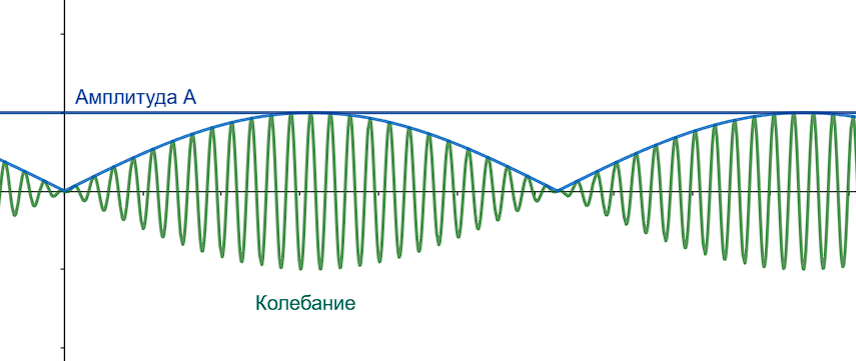
\includegraphics[width=13cm]{physics2/images/physics2_2025_03_17_2}
\end{center}

Предположим, что имеются две взаимно перпендикулярные векторные величины $x$ и $y$, изменяющиеся по закону:
$\vec x = \vec e_x A \cos \omega t, \qquad \vec y = \vec e_y B \cos (\omega t + \alpha)$

Здесь $e_x, e_y$ - орты координатных осей, $A, B$ - амплитуды

$\cos \omega t = \frac{x}{A}, \qquad \sin \omega t = \pm \sqrt{1 - \frac{x^2}{A^2}}$

$\frac{y}{B} = \cos (\omega t + \alpha) = \cos \omega t \cdot \cos \alpha - \sin \omega t \cdot \sin \alpha = 
\frac{x}{A} \cos \alpha \mp \sin \alpha \cdot \sqrt{1 - \frac{x^2}{A^2}}$

Немного преобразив выражение, получаем уравнение эллипса: $\frac{x^2}{A^2} + \frac{y^2}{B^2} - \frac{2xy}{AB} \cos \alpha = \sin^2 \alpha$

При $\alpha = 0$ результирующее движение является гармоническим колебанием вдоль прямой $y = \frac{B}{A} x$,
при других - эллипсом

% картинка 

При почти одинаковых частотах движение происходит по видоизменяющейся кривой. При разных частотах получаются фигуры Лиссажу

\subsection{Затухающие колебания}

Во всякой реальной колебательной системе всегда имеется либо сила трения, либо активное электрическое сопротивление,
действие которых приводит к уменьшению энергии системы 

Для пружинного маятника в вязкой среде получаем $m \ddot x = -kx - r\dot x$ или $\ddot x + 2 \beta \dot x + \omega^2_0 x = 0$

Ища решения в виде $x(t) = u(t) e^{\beta t}$, получаем $\ddot u + (\omega^2_0 - \beta^2) u = 0$

При $\omega_0 > \beta$ получим $\omega \equiv \sqrt{\omega^2 - \beta^2}$ и $\ddot u + \omega^2 u = 0$

Из этого $u = A_0 \cos (\omega t + \alpha)$, а $x(t) = A_0 e^{\beta t} \cos (\omega t + \alpha)$

Скорость затухания колебаний определяется величиной $\beta$, которую называют коэффициентом затухания. 
Также затухания можно характеризовать декрементом затухания $\lambda = \ln \frac{A(t)}{A(t + T)} = \beta T$

За время $\tau = \frac{T}{\lambda}$, за которое амплитуда уменьшается в $e$ раз, система успевает совершить $N_\tau = \frac{\tau}{T}$
колебаний

Также применяется величина добротности колебательной системы $Q = \frac{\pi}{\lambda}$

В электрическом колебательном контуре получаем $2\beta \equiv \frac{R}{L}$ и $\omega_0^2 \equiv \frac{1}{LC}$

$\ddot q + 2\beta \dot q + \omega^2_0 q = 0$

Здесь $\lambda = \frac{R}{2L} \cdot \frac{2\pi}{\omega} = \frac{R\pi}{L \omega}$, $Q = \frac{L\omega}{R}$


\subsection{Вынужденные колебания}

Пусть механическая колебательная система подвергается действию
внешней силы, изменяющейся со временем по гармоническому закону: $F_x = F_0 \cos \omega t$

Тогда $m\ddot{x} + r\dot{x} + kx = F_0 \cos(\omega t)$

Установившееся решение: $x(t) = \frac{F_0}{\sqrt{(k - m\omega^2)^2 + (r\omega)^2}} \cos(\omega t - \phi)$,
где $\phi = \arctan\left(\frac{r\omega}{k - m\omega^2}\right)$ — сдвиг фазы. 

Резонанс возникает при частоте: $\omega_{\text{рез}} = \sqrt{\omega_0^2 - 2\beta^2}$

Добротность определяет остроту резонанса: $Q = \frac{\omega_0}{2\beta}$.
